\section{Model2DRigid\-Chain  Class Reference}
\label{classModel2DRigidChain}\index{Model2DRigidChain@{Model2DRigid\-Chain}}
A 2D kinematic chain of bodies. 


{\tt \#include $<$model2d.h$>$}

Inheritance diagram for Model2DRigid\-Chain::\begin{figure}[H]
\begin{center}
\leavevmode
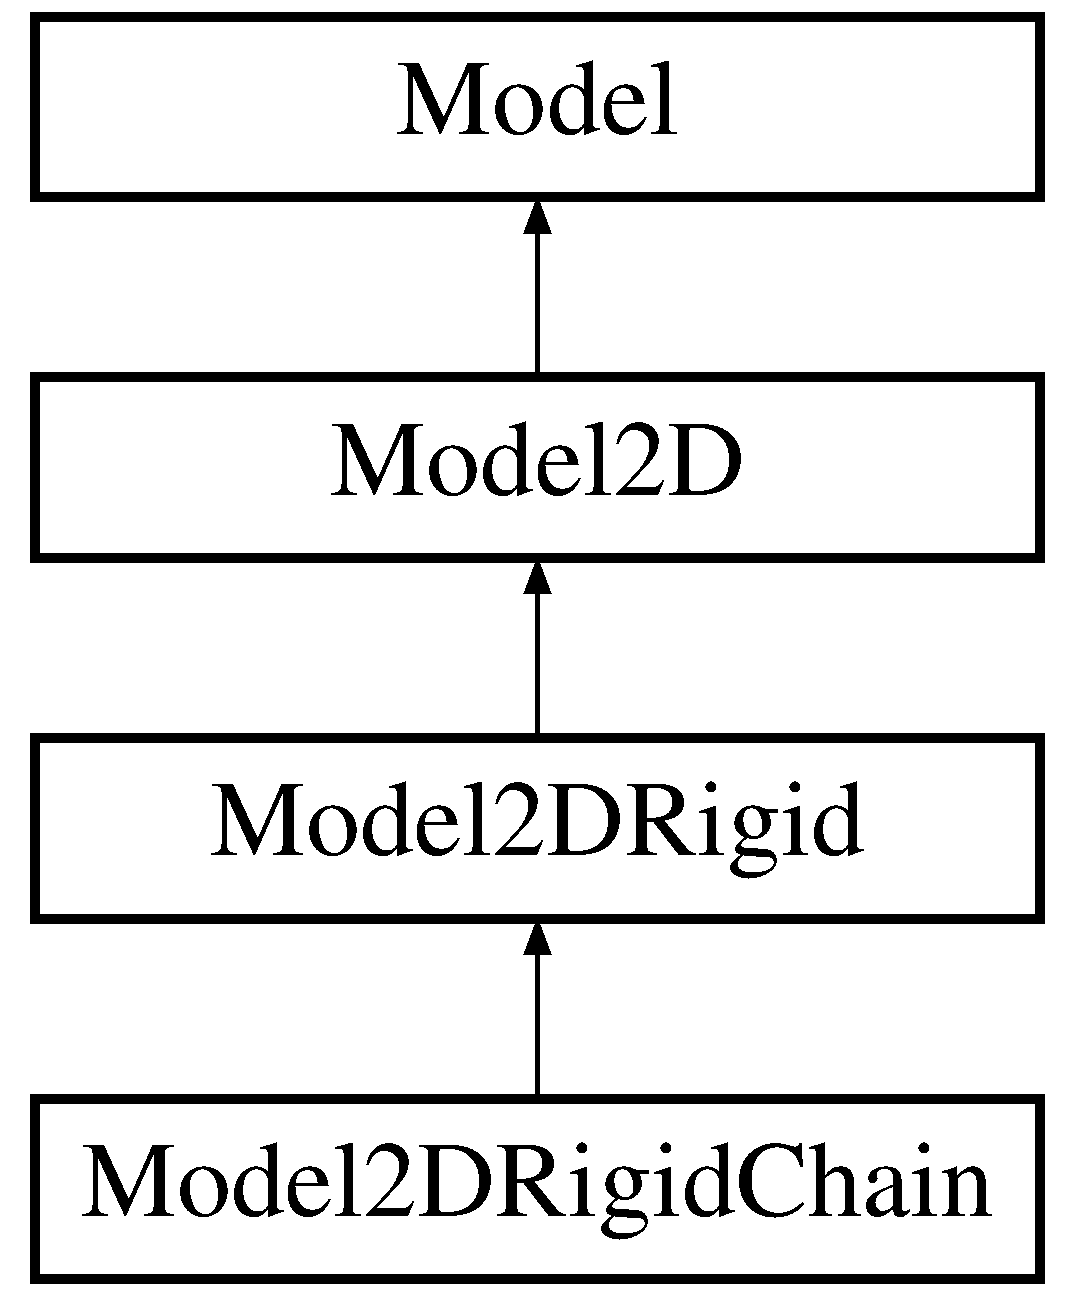
\includegraphics[height=4cm]{classModel2DRigidChain}
\end{center}
\end{figure}
\subsection*{Public Methods}
\begin{CompactItemize}
\item 
{\bf Model2DRigid\-Chain} (string path)
\item 
virtual {\bf $\sim$Model2DRigid\-Chain} ()
\item 
virtual {\bf MSLVector} {\bf State\-To\-Configuration} (const {\bf MSLVector} \&x)
\begin{CompactList}\small\item\em A method that converts a {\bf Model} {\rm (p.\,\pageref{classModel})} state in to a {\bf Geom} {\rm (p.\,\pageref{classGeom})} configuration.\item\end{CompactList}\item 
virtual {\bf MSLVector} {\bf State\-Transition\-Equation} (const {\bf MSLVector} \&x, const {\bf MSLVector} \&u)
\begin{CompactList}\small\item\em The state transition equation, or equations of motion, xdot=f(x,u).\item\end{CompactList}\item 
virtual {\bf MSLVector} {\bf Linear\-Interpolate} (const {\bf MSLVector} \&x1, const {\bf MSLVector} \&x2, const double \&a)
\begin{CompactList}\small\item\em Linearly interpolate two state while respecting topology.\item\end{CompactList}\item 
virtual double {\bf Metric} (const {\bf MSLVector} \&x1, const {\bf MSLVector} \&x2)
\begin{CompactList}\small\item\em A distance metric, which is Euclidean in the base class.\item\end{CompactList}\item 
virtual bool {\bf Satisfied} (const {\bf MSLVector} \&x)
\begin{CompactList}\small\item\em Test whether global state-space constraints are satisfied.\item\end{CompactList}\end{CompactItemize}
\subsection*{Public Attributes}
\begin{CompactItemize}
\item 
int {\bf Num\-Bodies}
\begin{CompactList}\small\item\em Number of bodies in the chain.\item\end{CompactList}\item 
{\bf MSLVector} {\bf A}
\begin{CompactList}\small\item\em The distances between joints (\char`\"{}a\char`\"{} parameters in kinematics).\item\end{CompactList}\item 
double {\bf Stop\-Angle}
\begin{CompactList}\small\item\em The default joint limits (must be in 0,PI).\item\end{CompactList}\end{CompactItemize}


\subsection{Detailed Description}
A 2D kinematic chain of bodies.



\subsection{Constructor \& Destructor Documentation}
\index{Model2DRigidChain@{Model2DRigid\-Chain}!Model2DRigidChain@{Model2DRigidChain}}
\index{Model2DRigidChain@{Model2DRigidChain}!Model2DRigidChain@{Model2DRigid\-Chain}}
\subsubsection{\setlength{\rightskip}{0pt plus 5cm}Model2DRigid\-Chain::Model2DRigid\-Chain (string {\em path} = \char`\"{}\char`\"{})}\label{classModel2DRigidChain_a0}


\index{Model2DRigidChain@{Model2DRigid\-Chain}!~Model2DRigidChain@{$\sim$Model2DRigidChain}}
\index{~Model2DRigidChain@{$\sim$Model2DRigidChain}!Model2DRigidChain@{Model2DRigid\-Chain}}
\subsubsection{\setlength{\rightskip}{0pt plus 5cm}Model2DRigid\-Chain::$\sim$Model2DRigid\-Chain ()\hspace{0.3cm}{\tt  [inline, virtual]}}\label{classModel2DRigidChain_a1}




\subsection{Member Function Documentation}
\index{Model2DRigidChain@{Model2DRigid\-Chain}!LinearInterpolate@{LinearInterpolate}}
\index{LinearInterpolate@{LinearInterpolate}!Model2DRigidChain@{Model2DRigid\-Chain}}
\subsubsection{\setlength{\rightskip}{0pt plus 5cm}{\bf MSLVector} Model2DRigid\-Chain::Linear\-Interpolate (const {\bf MSLVector} \& {\em x1}, const {\bf MSLVector} \& {\em x2}, const double \& {\em a})\hspace{0.3cm}{\tt  [virtual]}}\label{classModel2DRigidChain_a4}


Linearly interpolate two state while respecting topology.

If a=0, then x1 is returned; if a=1, then x2 is returned. All intermediate values of \$a $\backslash$in [0,1]\$ yield intermediate states. This method is defined by {\bf Model} {\rm (p.\,\pageref{classModel})}. 

Reimplemented from {\bf Model2DRigid} {\rm (p.\,\pageref{classModel2DRigid_a4})}.\index{Model2DRigidChain@{Model2DRigid\-Chain}!Metric@{Metric}}
\index{Metric@{Metric}!Model2DRigidChain@{Model2DRigid\-Chain}}
\subsubsection{\setlength{\rightskip}{0pt plus 5cm}double Model2DRigid\-Chain::Metric (const {\bf MSLVector} \& {\em x1}, const {\bf MSLVector} \& {\em x2})\hspace{0.3cm}{\tt  [virtual]}}\label{classModel2DRigidChain_a5}


A distance metric, which is Euclidean in the base class.



Reimplemented from {\bf Model2DRigid} {\rm (p.\,\pageref{classModel2DRigid_a5})}.\index{Model2DRigidChain@{Model2DRigid\-Chain}!Satisfied@{Satisfied}}
\index{Satisfied@{Satisfied}!Model2DRigidChain@{Model2DRigid\-Chain}}
\subsubsection{\setlength{\rightskip}{0pt plus 5cm}bool Model2DRigid\-Chain::Satisfied (const {\bf MSLVector} \& {\em x})\hspace{0.3cm}{\tt  [virtual]}}\label{classModel2DRigidChain_a6}


Test whether global state-space constraints are satisfied.



Reimplemented from {\bf Model} {\rm (p.\,\pageref{classModel_a4})}.\index{Model2DRigidChain@{Model2DRigid\-Chain}!StateToConfiguration@{StateToConfiguration}}
\index{StateToConfiguration@{StateToConfiguration}!Model2DRigidChain@{Model2DRigid\-Chain}}
\subsubsection{\setlength{\rightskip}{0pt plus 5cm}{\bf MSLVector} Model2DRigid\-Chain::State\-To\-Configuration (const {\bf MSLVector} \& {\em x})\hspace{0.3cm}{\tt  [virtual]}}\label{classModel2DRigidChain_a2}


A method that converts a {\bf Model} {\rm (p.\,\pageref{classModel})} state in to a {\bf Geom} {\rm (p.\,\pageref{classGeom})} configuration.



Reimplemented from {\bf Model2DRigid} {\rm (p.\,\pageref{classModel2DRigid_a6})}.\index{Model2DRigidChain@{Model2DRigid\-Chain}!StateTransitionEquation@{StateTransitionEquation}}
\index{StateTransitionEquation@{StateTransitionEquation}!Model2DRigidChain@{Model2DRigid\-Chain}}
\subsubsection{\setlength{\rightskip}{0pt plus 5cm}{\bf MSLVector} Model2DRigid\-Chain::State\-Transition\-Equation (const {\bf MSLVector} \& {\em x}, const {\bf MSLVector} \& {\em u})\hspace{0.3cm}{\tt  [virtual]}}\label{classModel2DRigidChain_a3}


The state transition equation, or equations of motion, xdot=f(x,u).



Reimplemented from {\bf Model2DRigid} {\rm (p.\,\pageref{classModel2DRigid_a3})}.

\subsection{Member Data Documentation}
\index{Model2DRigidChain@{Model2DRigid\-Chain}!A@{A}}
\index{A@{A}!Model2DRigidChain@{Model2DRigid\-Chain}}
\subsubsection{\setlength{\rightskip}{0pt plus 5cm}{\bf MSLVector} Model2DRigid\-Chain::A}\label{classModel2DRigidChain_m1}


The distances between joints (\char`\"{}a\char`\"{} parameters in kinematics).

\index{Model2DRigidChain@{Model2DRigid\-Chain}!NumBodies@{NumBodies}}
\index{NumBodies@{NumBodies}!Model2DRigidChain@{Model2DRigid\-Chain}}
\subsubsection{\setlength{\rightskip}{0pt plus 5cm}int Model2DRigid\-Chain::Num\-Bodies}\label{classModel2DRigidChain_m0}


Number of bodies in the chain.

\index{Model2DRigidChain@{Model2DRigid\-Chain}!StopAngle@{StopAngle}}
\index{StopAngle@{StopAngle}!Model2DRigidChain@{Model2DRigid\-Chain}}
\subsubsection{\setlength{\rightskip}{0pt plus 5cm}double Model2DRigid\-Chain::Stop\-Angle}\label{classModel2DRigidChain_m2}


The default joint limits (must be in 0,PI).



The documentation for this class was generated from the following files:\begin{CompactItemize}
\item 
{\bf model2d.h}\item 
{\bf model2d.C}\end{CompactItemize}
